\chapter{Ermittlung der Funkreichweite}
\label{ch:Reichweite}
Die Ermittelung der Reichweite dient dazu, das nötige Sendeintervall zu bestimmen.
Die Reichweite wurde bisher als 50 Meter angenommen, das Sendeintervall dementsprechend auf 5 Sekunden gesetzt.
In dieser Zeit kann ein Mitarbeiter maximal 42 Meter bei einer Geschwindigkeit von 30 km/h bewegen. 
Für den anschließenden Vergleich sollen jedoch realistische Bedingungen, mit einem für die Funkcharakteristik des Tunnels angepassten Sendeintervall, geschaffen werden.

\section{Umgebung}
Für die Tests wurde ein LN-862 Access Point von der Firma Lancom zur Verfügung gestellt.
Dieser wurde am hinteren Ende einer Tunnelbohrmaschine montiert.\\
Die Tunnelbohrmaschine befindet sich in der Tunnelbaustelle Rastatt. 
Der Durchmesser des Bahntunnels beträgt 9 Meter, das Ende der Tunnelbohrmaschine befand zum Zeitpunkt der Messungen circa 2 Kilometer weit im Tunnel.\\
Der AP konnte aufgrund des geringen Platzangebots und den wenigen zur Verfügung stehenden Steckdosen nicht frei platziert werden.
Er wurde deshalb unter der ersten stählernen Treppe platziert, diese beeinträchtigt natürlich das Signal.
Da es aber üblich ist IT-Gerätschaften, wie die derzeit verwendeten Bluetooth-Basisstationen, in Metallboxen zu verstauen um sie vor äußeren Einflüssen zu schützen, ist eine gewisse Abschirmung durchaus realitätsnah.
Die Platzierung des AP ist auf Abb. \ref{fig:tunnelmark} eingezeichnet.\\
Der Versuchsaufbau für Bluetooth ist identisch, es wurde jedoch ein Raspberry Pi Zero W als Basisstation verwendet. 
Der Pi Zero W wurde an der selben Position wie der LN-862 montiert, Abb. \ref{fig:applacement} zeigt beide Basisstationen.

\begin{figure}[h]
  \centering
	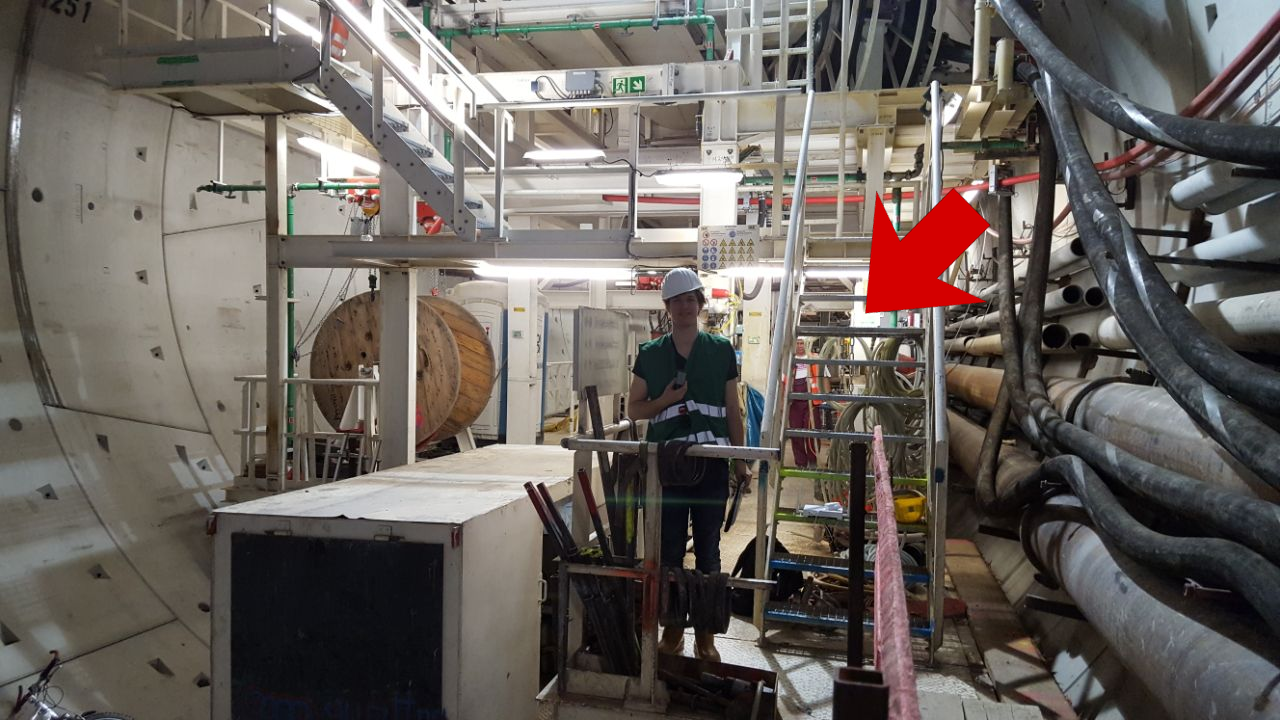
\includegraphics[width=\textwidth]{images/tunnelmark.png}
  \caption{Ende der Tunnelbohrmaschine, Pfeil markiert Platzierung des Acces Point hinter der Treppe.}
  \label{fig:tunnelmark}
\end{figure}

\begin{figure}[h]
  \centering
	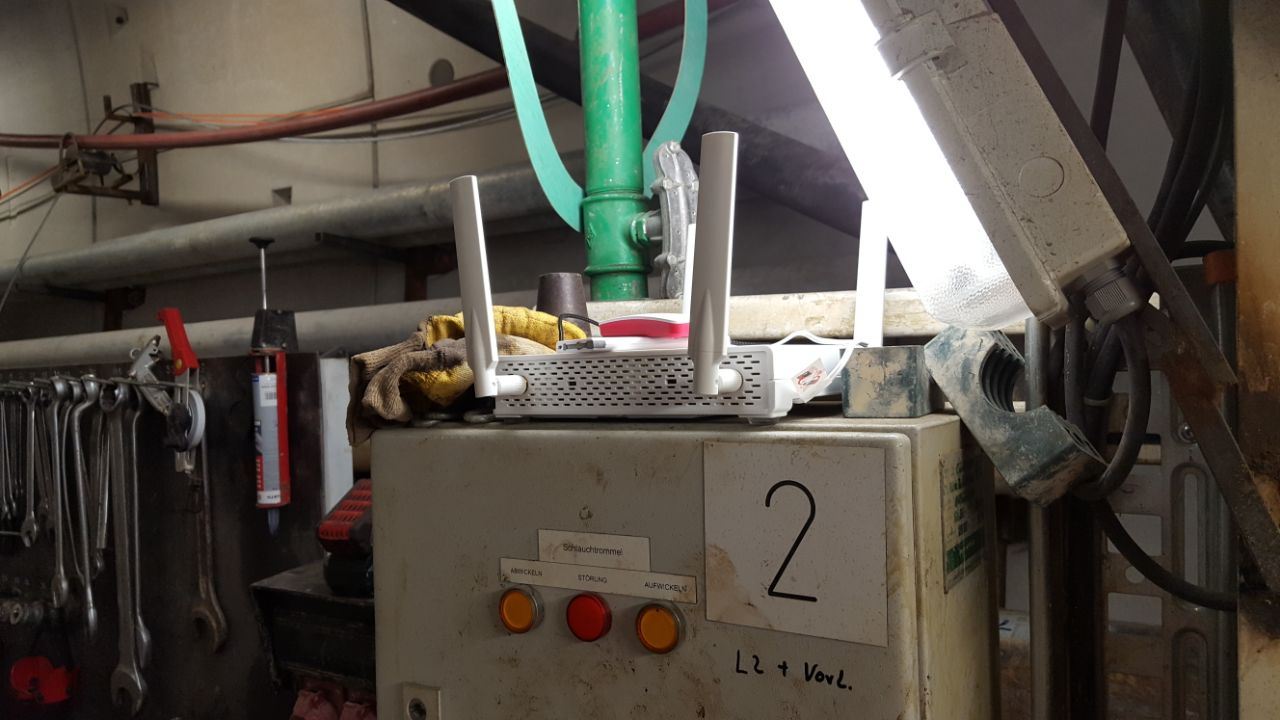
\includegraphics[width=\textwidth]{images/applacement.jpg}
  \caption{LN-862 im Tunnel, darauf liegt der Pi Zero W.}
  \label{fig:applacement}
\end{figure}

\section{Methodik}
Die Reichweite in zwei Richtungen geprüft.
Zum einen in Richtung des bereits fertig gebohrten Tunnels, hier blockiert nur wenig Stahl das Signal. 
Lediglich die Treppe, unter der der AP montiert wurde, stellt ein Hindernis dar.
Zum anderen wurde die Reichweite in Richtung des Vortriebs geprüft.
Dabei stellen eine stählerne Zwischendecke und große Container Hindernisse dar.\\
Außerdem wird die Abschrimung durch ein Gehäuse getestet.
Dazu wurde eine stabile Plastikbox verwendet, leider konnte diese für den Versuch mit dem Bluetooth-Tag nicht vollends geschlossen werden.\\
Für die Messung wurde der Körper zwischen Tag und Basisstation gebracht und ein Tag wurde dann als "außer Reichweite" angesehen, wenn versendete Pakete des Tags nicht mehr bei der Basisstation ankamen.
In jedem Fall war es möglich durch das Entfernen des körperlichen Hindernisses wieder eine Verbindung herzustellen.\\
Zur Bestimmung der Distanz wurden die Tübbinge verwendet, dies sind Schalungselemente im Tunnel.
Im Tunnel Raststatt sind diese fortlaufend nummeriert und genau zwei Meter breit, die Messungen sind deshalb ebenfalls in zwei Meter Schritten angegeben.

\section{Ergebnisse}
Tabelle \ref{table:rangewifi} zeigt die Ergebnisse für die zwei verwendeten ESP8266 Module.
Es wurde jeweils mit und ohne Gehäuse gemessen und in jede der beiden beschriebenen Richtungen.
Wenige Hindernisse bezeichnet dabei die Richtung des bereits fertig gebohrten Tunnels, viele Hindernisse die Richtung des Vortriebs.

\begin{table}[h]
	\centering
	\caption{Sendereichweite WLAN-basierter Tags}
	\label{table:rangewifi}
	\begin{tabular}{p{3.5cm}|p{3cm}|p{3.5cm}|p{3cm}}
		Verwendetes Modul & Aufbau & Strecke & Maximale Sendereichweite \\
		\hline
		ESP-12E & Offen & Wenige Hindernisse & 84m \\
		ESP-12E & In Gehäuse & Wenige Hindernisse & 74m \\
		ESP-12E & Offen & Viele Hindernisse & 26m \\
		ESP-12E & In Gehäuse & Viele Hindernisse & 30m \\
		\hline
		ESP-12F & Offen & Wenige Hindernisse & 88m \\
		ESP-12F & In Gehäuse & Wenige Hindernisse & 88m \\
		ESP-12F & Offen & Viele Hindernisse & 32m \\
		ESP-12F & In Gehäuse & Viele Hindernisse & 32m \\
	\end{tabular}
\end{table}

Tabelle \ref{table:rangeblue} zeigt die Ergebnisse für den nRF52.
Für diesen sind keine Ergebnisse mit geschlossenem Gehäuse aufgeführt, denn das Gehäuse ließ sich für diesen Prototyp nicht schließen.
Das lose Auflegen des Deckels führte zu keiner Veränderung bei der Reichweite.

\begin{table}[h]
	\centering
	\caption{Sendereichweite Bluetooth-basierter Tags}
	\label{table:rangeblue}
	\begin{tabular}{p{3.5cm}|p{3cm}|p{3.5cm}|p{3cm}}
		Verwendetes Modul & Aufbau & Strecke & Maximale Sendereichweite \\
		\hline
		nRF52 & Offen & Wenige Hindernisse & 32m \\
		nRF52 & Offen & Viele Hindernisse & 14m \\
	\end{tabular}
\end{table}

\section{Bewertung}
\label{ch:Reichweite:sec:bewertung}
Das ESP-12F Modul hatte in jedem der vier Testszenarien eine höhere Reichweite als das ESP-12E, es ist daher im weiteren Verlauf zu bevorzugen.\\
Die bisher angenommenen 50 Meter Reichweite sind für dieses Modul deutlich zu vorsichtig geschätzt. 
Um die gemessenen 88 Meter bei 30 km/h zu durchqueren benötigte ein Mitarbeiter circa 10,5 Sekunden, bei einem Sendeintervall von zehn Sekunden finden demnach zwei Sendevorgänge beim durchqueren des Einflussbereichs eines APs statt.
Da eine zuverlässige Erkennung von Bereichswechseln gefordert wurde, sollte das Sendeintervall konservativer auf acht Sekunden gesetzt werden.\\
Für die Teststrecke mit vielen Hindernissen wurden geringere Reichweiten gemessen, eine solche Teststecke findet sich aber nur auf der Tunnelbohrmaschine, welche nur zu Fuß begangen werden kann. 
Geht man von einer maximalen Bewegungsgeschwindigkeit von zehn km/h für eine laufende Person aus durquerte diese in acht Sekunden 22 Meter, also deutlich weniger als die gemessenen 32 Meter.\\
Auch die Reichweite des nRF52 war größer als erwartet, da dieser jedoch die geforderten drei Jahre Laufzeit auch bei einem Sendeintervall von einer Sekunde erfüllt kann die unverändert bleiben.
